\documentclass{beamer}
\usetheme[language=italian,
		  bullet=triangle,
		  color=blue,
		  titleline=true,
		  notshowauthor=true,
		  notshowtitle=true
         ]{TorinoTh}
\setbeamertemplate{caption}[numbered] % per avere fig. numerate nelle caption
\makeatletter
\renewcommand{\fnum@figure}{Fig. \thefigure} %per avere fig. invece che figura
\makeatother
\usepackage[beamer,customcolors]{hf-tikz}
\usepackage{graphicx}
\usepackage[font={footnotesize}]{caption}
\usepackage{wrapfig}

\hfsetfillcolor{alerted text.fg!10}
\hfsetbordercolor{alerted text.fg}

\begin{center}
\small Alma Mater Studiorum - Università di Bologna
\end{center}
\begin{center}
\small Scuola di Scienze - Corso di Laurea in Informatica
\end{center}

\author{Simone Preite}
\rel{Renzo Davoli}
\title{VSNLib: un'interfaccia unica di configurazione per stack virtuali tramite pacchetti netlink}
\ateneo{Università di Bologna}

%\date{Sessione II\\
%Anno Accademico 2016/2017\\ \\
%11 ottobre 2017} lo voglio fare uguale al frontespizio della tesi TODO

\date{20 dicembre 2017}

\begin{document}

\titlepageframe % Specific command


\begin{frame}[fragile]{Introduzione}
Il lavoro di tesi riguarda lo sviluppo di una libreria utile per facilitare la configurazione degli stack di rete virtuali  agli sviluppatori che intendono farne uso.
\end{frame}

\begin{frame}[fragile]{IPv6 vs IPv4}

\begin{itemize}
    \item IPv4 \`e insufficiente per fronteggiare la necessit\`a di nuovi indirizzi;
    \item Il numero di nodi sulla rete in continua ascesa, necessitano di nuovi indirizzi;
    \item IPv6: soluzione proposta gi\`a da diversi anni ma non ancora di largo utilizzo.
\end{itemize}
\begin{table}[h]                        %ambiente tabella
                                        %(serve per avere la legenda)
\begin{center}                          %centra nella pagina la tabella
\begin{tabular}{r|c|c|c}                  %tre colonne con righe verticali
                                        %   prodotte con |
\hline
IP $\langle version \rangle$ & 80 bit & 16 bit & 32 bit\\
\hline \hline                         %inserisce due righe orizzontali
$IPv4$ &   &   & $192.168.1.2$\\           %& separa le colonne e con
\hline                                  %inserisce una riga orizzontale
$IPv6$ & $00000000.00000000.0000$ & $FFFF$ & $192.168.1.2$\\           %  \\ va a capo
\hline                                  %inserisce una riga orizzontale
$IPv6$ & $00000000.00000000.0000$ & $FFFF$ & $C0A80102$\\
\hline                           %inserisce due righe orizzontali
\end{tabular}
\caption[IPv4 to IPv6 conversion]{rappresentazione di un indirizzo IPv4 in IPv6}\label{tab:IPv4toIPv6}
\end{center}
\end{table}
\end{frame}


\begin{frame}[fragile]{IoT}

\begin{columns}[T]
\begin{column}{.30\textwidth}
\newline
\begin{itemize}
    \item Connessione dispositivi comuni alla rete;\newline
		\item Aumento esponenziale dei nodi.\newline

\end{itemize}

\end{column}%
\hfill%
\begin{column}{.50\textwidth}
    \begin{figure}[t!]
    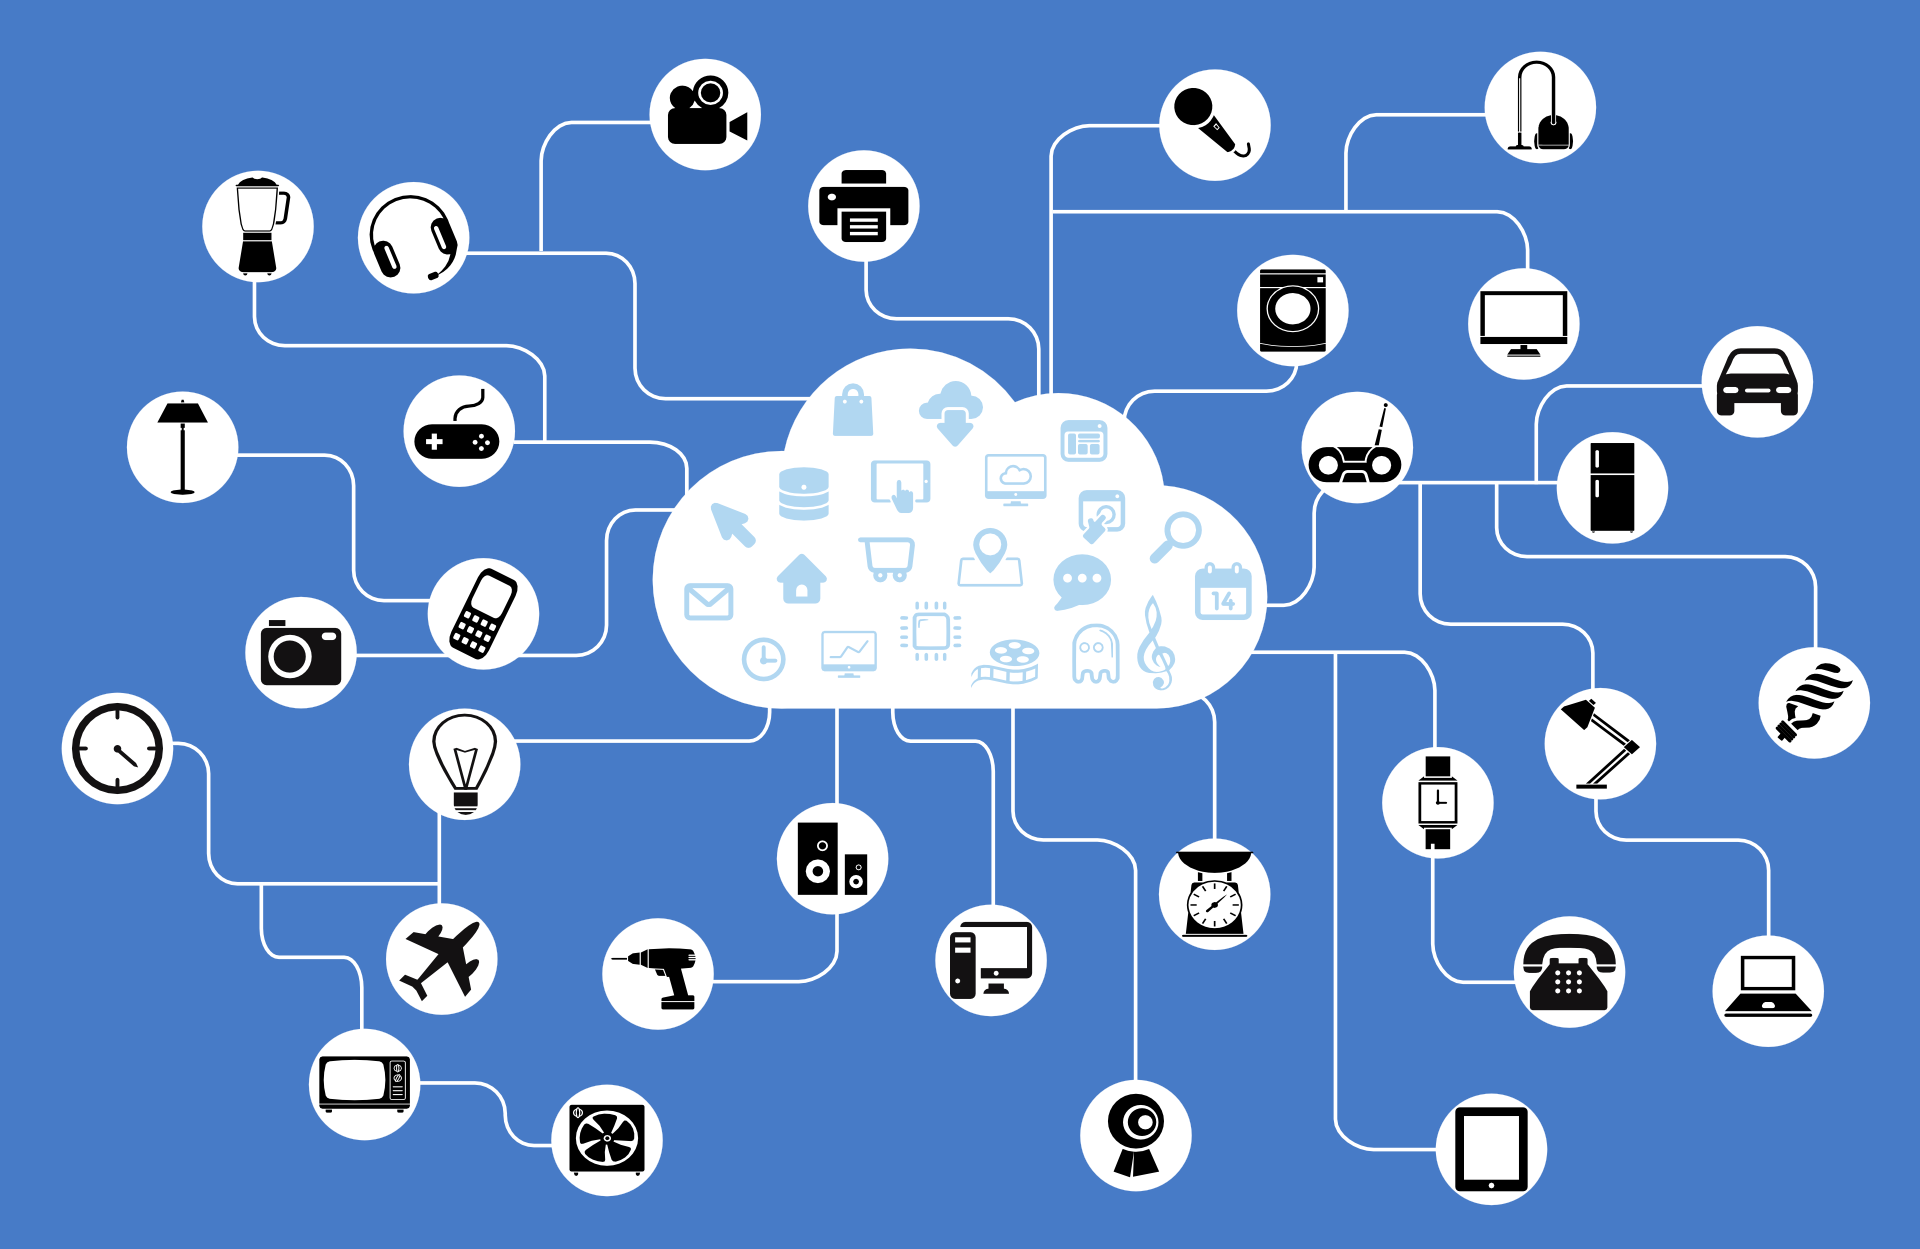
\includegraphics[scale=.08]{img/IoT.png}
    \caption{Internet of Things}
    \centering

\end{figure}
\end{column}%non mi piacciono le immagini
\end{columns}
\end{frame}

\begin{frame}[fragile]{IoTh}
	\begin{columns}[T]
	\begin{column}{.40\textwidth}
	    \begin{figure}[t!]
	    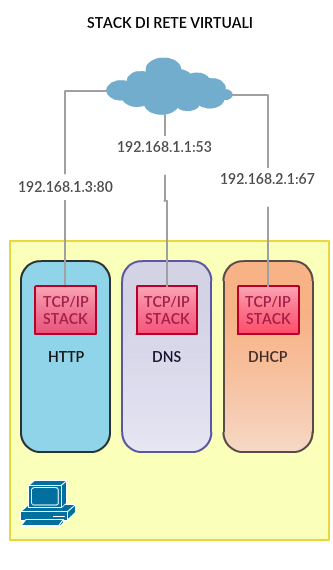
\includegraphics[scale=0.35]{img/new_stack.png}
	    \caption{Internet of Things}
	    \centering

	\end{figure}
	\end{column}%non mi piacciono le immagini
	\hfill%
	\begin{column}{.60\textwidth}
	\newline
	\begin{itemize}
	    \item Connessione di processi direttamente alla rete;\newline
			\item Possibile grazie al gran numero di indirizzi IPv6;\newline
			\item Paradigma simile alla telefonia mobile rispetto a quella fissa;\newline
			\item \`E possibile trasferire processi da un capo all'altro del mondo senza problemi di indirizzamento e senza che il client si renda conto di nulla.\newline
	\end{itemize}

	\end{column}%
	\end{columns}
\end{frame}

\begin{frame}[fragile]{Stack Virtuali}


		\begin{columns}[T]
		\begin{column}{.40\textwidth}
			\begin{minipage}[c][0.6\textheight]{\linewidth}
		 \begin{figure}[t!]
		    
\includegraphics[scale=0.2]{img/lwip}
			    \caption{LWIP}
			\end{figure}
				\begin{figure}[t!]
		    
\includegraphics[scale=0.2]{img/picoTCP.png}
		    \caption{picoTCP}
			\end{figure}
\end{minipage}
		    \centering

		\end{column}
		\hfill%
		\begin{column}{.60\textwidth}
		\newline
		\begin{itemize}
		    \item PicoTCP\newline
				\item LightWeight IP (LWIP)\newline
				\item LightWeight IPv6 (LWIPv6)\newline

		\end{itemize}

		\end{column}%
		\end{columns}
		\vspace{1em}

		progetti di stack esistenti che permettono ai processi di comunicare tramite indirizzo personale

\end{frame}

\begin{frame}[fragile]{VSNLib}

Perch\`e:\newline
\begin{itemize}
    \item Uniformit\`a dell'interfaccia di configurazione;
    \item Facilitare gli sviluppatori che si approcciano a questa tecnologia;
    \item Immediatezza: non \`e necessario studiare come la libreria debba essere configurata.
\end{itemize}
\vspace{1em}
Si vuole dare la possibilit\`a al programmatore di usare programmi come\\\vspace{1em} \centering{\textit{\textbf{ip addr add 10.0.0.1/24 dev tap0}}} \\
\vspace{1em}
per configurare lo stack, come farebbe all'interno di un sistema linux.
\end{frame}

\begin{frame}[fragile]{Netlink}
	\begin{figure}[t!]
	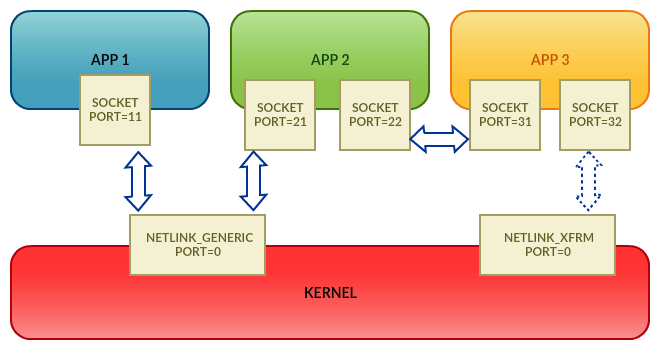
\includegraphics[scale=0.4]{img/netlink_comunication}
	\caption{netlink}
	\end{figure}
	\vspace{1em}
Netlink \`e un sistema di Inter Process Comminication (IPC), ovvero permette ai processi di scambiarsi messaggi.\\
Le porte utilizzate per la comunicazione sono create in funzione dei Process ID.\\
 %\begin{itemize}
    %\setlength\itemsep{2em}
    % \item Startup\newline
    % il client VNC viene eseguito in automatico all'avvio tramite creazione di desktop entry
%
  %   \item Indirizzo IP statico\newline
  %   viene abilitato modificando il file di configurazione del demone dhcpcd
  %   \item Blank screen\newline
  %   viene disabilitato agendo sul file di configurazione di LightDM, il display manager
 %\end{itemize}

 %%TODO magari dividere in due colonne e a dx mettere i listings...
\end{frame}

\begin{frame}[fragile]{Flusso}
 \begin{itemize}
   \setlength\itemsep{2em}
	 \item Pre-VSNLib:
	 \vspace{0.5em}
			\begin{itemize}
			\setlength\itemsep{0.5em}
			\item Cattura della system call (sendto)
			\end{itemize}
     \item Sequenza:
     \vspace{0.5em}
        \begin{itemize}
        \setlength\itemsep{0.5em}
        \item Init
        \item Cattura pacchetto
        \item Core (gestione e decodifica)
        \item Chiamata alla funzione del modulo
				\item Modulo
				\item Core (risposta)
        \end{itemize}

 \end{itemize}
\end{frame}

\begin{frame}[fragile]{Core}
	\begin{itemize}
			\item Inizializza la libreria caricando il modulo per lo stack in uso;\newline
			\item ``Handle'' per il passaggio del pacchetto netlink;\newline
			\item Decode del pacchetto;\newline
			\item Chiamata alla funzione del modulo per l'azione richiesta;\newline
			\item Creazione del netlink di risposta.

	\end{itemize}
\end{frame}

\begin{frame}[fragile]{Moduli}
	\begin{itemize}
      \item Stessa struttura;\newline
      \item Strato di compatibilit\`a con le funzioni particolari degli stack;\newline
      \item Possibilit\`a di creare nuovi moduli per aumentare la compatibilit\`a con altri stack.

  \end{itemize}
\end{frame}

\begin{frame}[fragile]{Test}
	\begin{itemize}
\item Il test \`e un client netcat il cui stack \`e stato configurato tramite un pacchetto netlink;\\
\item Sono visibili i feedback di risposta e la corretta configurazione dello stack \`e dimostrata dal fatto che il client riesce a comunicare con il server.
\end{itemize}
\begin{figure}[t!]
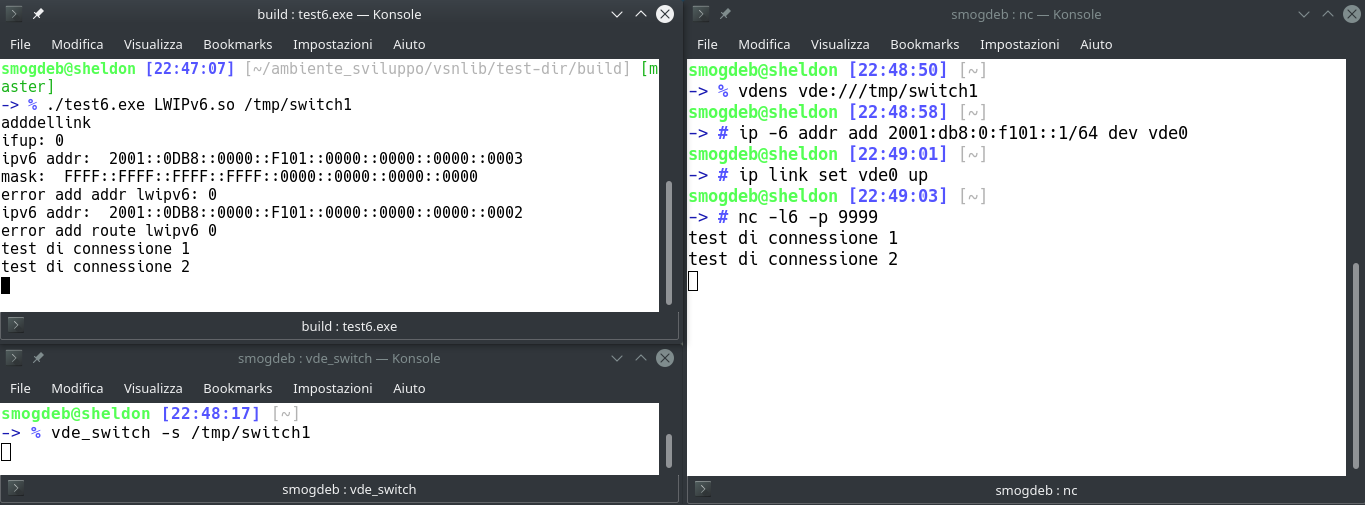
\includegraphics[scale=0.28]{img/test6_b}
\caption{netlink}
\end{figure}
\end{frame}

\begin{frame}[fragile]{Conclusioni}
 \begin{itemize}
     \item I test effetuati indicano la riuscita della configurazione;\newline
     \item VSNLib \`e ancora un prototipo ma i risultati sono incoraggianti;\newline
     \item L'obiettivo finale \`e quello di avere una libreria completa e trasparente.
 \end{itemize}
\end{frame}


\begin{frame}[fragile]{Sviluppi Futuri}
 \begin{itemize}
	 	\item Aumento compatibilit\`a con gli stack esistenti, controllo e testing;\newline
		\item Sviluppo di moduli per eventuali nuovi stack;\newline
     \item Package Filtering: configurazione attraverso iptables.
 \end{itemize}
\end{frame}


\begin{frame}[c]

\begin{center}
\LARGE Grazie per l'attenzione\\
\end{center}
\end{frame}

%\begin{frame}[plain, noframenumbering]{Approfondimento:}

%\newline

%\begin{itemize}


%\end{itemize}
%\end{frame}



%\begin{frame}[plain, noframenumbering]{Approfondimento:}

%\begin{itemize}
%\end{itemize}
%\end{frame}

%\begin{frame}[plain, noframenumbering]{Approfondimento: }

%\begin{itemize}

%\end{itemize}

%\end{frame}





\end{document}
